\begin{frame}{Benchmark (1/4)}

\begin{itemize}\itemsep1em
\item
Test system:
\begin{itemize}
\item
Intel(R) Xeon(R) Platinum 8276 CPU @ 2.20GHz,
28 cores (56 threads),
1 TB RAM

\item
Matlab R2021a (Update 5) on CentOS 7 \\[0.5em]

\item
{\color{blue}
APA (1.0.0), Advanpix (4.8.5.14569), GEM (2.0.2), VPA (R2021a)}
\end{itemize}

\item
Tests with \lstinline|A = rand(N,N)| and \lstinline|b = A * ones(N,1)|:

\begin{itemize}
\item
Matrix-Matrix-Multiplication
$\quad$
\lstinline|A * A|

\item
LU-factorization
$\qquad\qquad\qquad$
\lstinline|[L,U] = lu (A)|

\item
Solve $Ax = b$
$\qquad\qquad\qquad\quad\;$
\lstinline|x = A \\ b|\\[0.5em]

\item
Precisions \cite[Chapter 3.1]{Muller2018}:

\begin{tabular}{|c|c|c|}
\hline
Name & Binary & Decimal\footnote{\scriptsize decimal precision
:= $\lfloor \text{binary precision} \times \log_{10}(2) \rfloor$,
see "bits2digits" in \url{http://www.holoborodko.com/pavel/mpfr/}.} \\
\hline\hline
"double"    &  53 & 15 \\
"quadruple" & 113 & 34 \\
"octuple"   & 237 & 71 \\
\hline
\end{tabular}

\end{itemize}

\end{itemize}

\end{frame}


\begin{frame}{Benchmark (2/4)}

\begin{columns}
\begin{column}{0.3\textwidth}
\begin{figure}
\centering
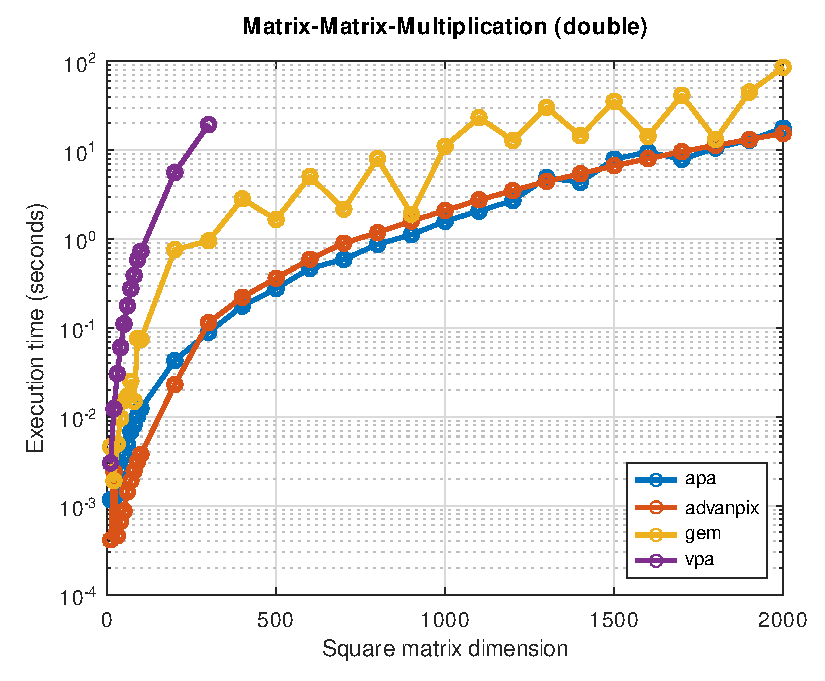
\includegraphics[width=1.0\linewidth]{res/data/2021-11-24_run-01-mmm-double-semilogy}
\end{figure}
\end{column}
\begin{column}{0.3\textwidth}
\begin{figure}
\centering
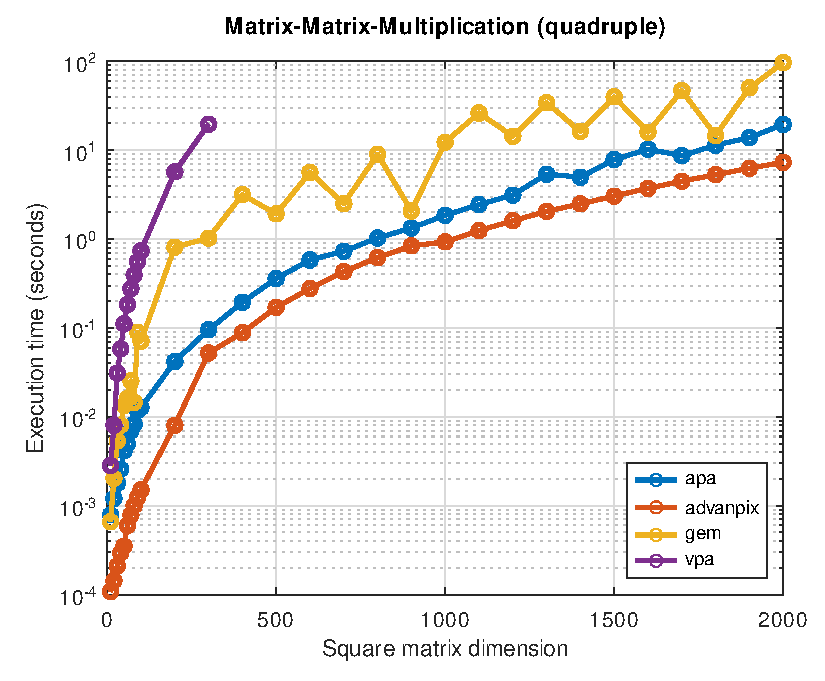
\includegraphics[width=1.0\linewidth]{res/data/2021-11-24_run-01-mmm-quadruple-semilogy}
\end{figure}
\end{column}
\begin{column}{0.3\textwidth}
\begin{figure}
\centering
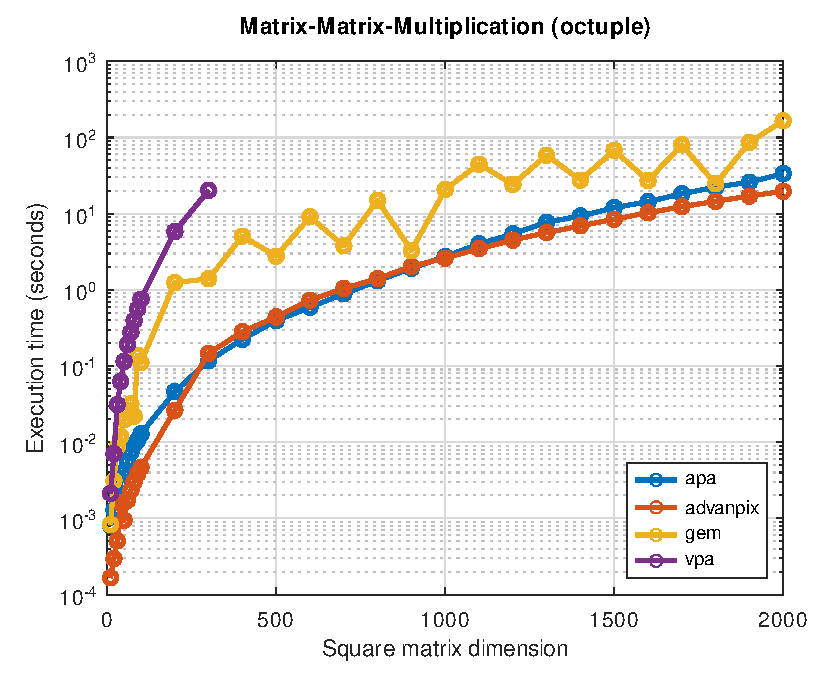
\includegraphics[width=1.0\linewidth]{res/data/2021-11-24_run-01-mmm-octuple-semilogy}
\end{figure}
\end{column}
\end{columns}

\end{frame}


\begin{frame}{Benchmark (3/4)}

\begin{columns}
\begin{column}{0.3\textwidth}
\begin{figure}
\centering
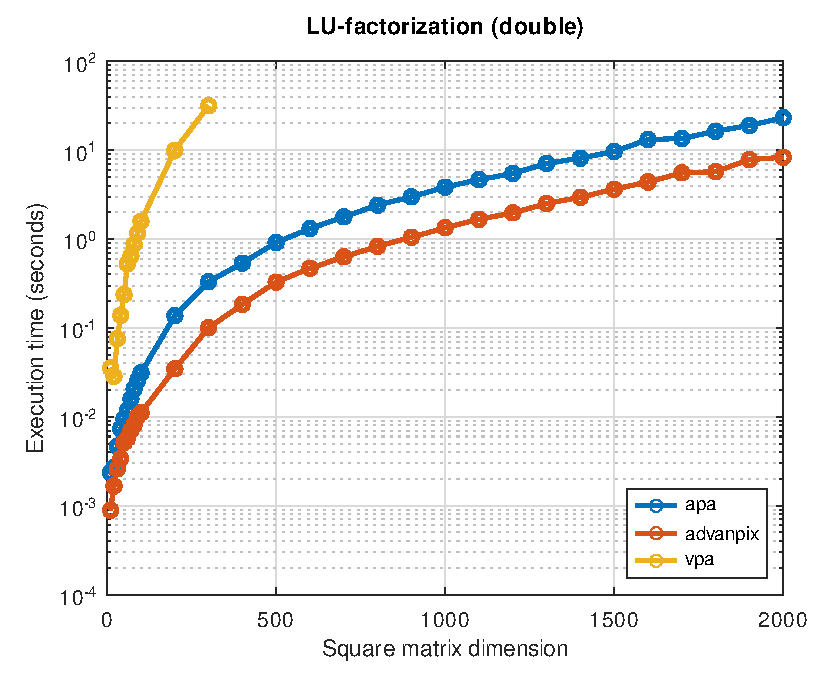
\includegraphics[width=1.0\linewidth]{res/data/2021-11-24_run-01-lu-double-semilogy}
\end{figure}
\end{column}
\begin{column}{0.3\textwidth}
\begin{figure}
\centering
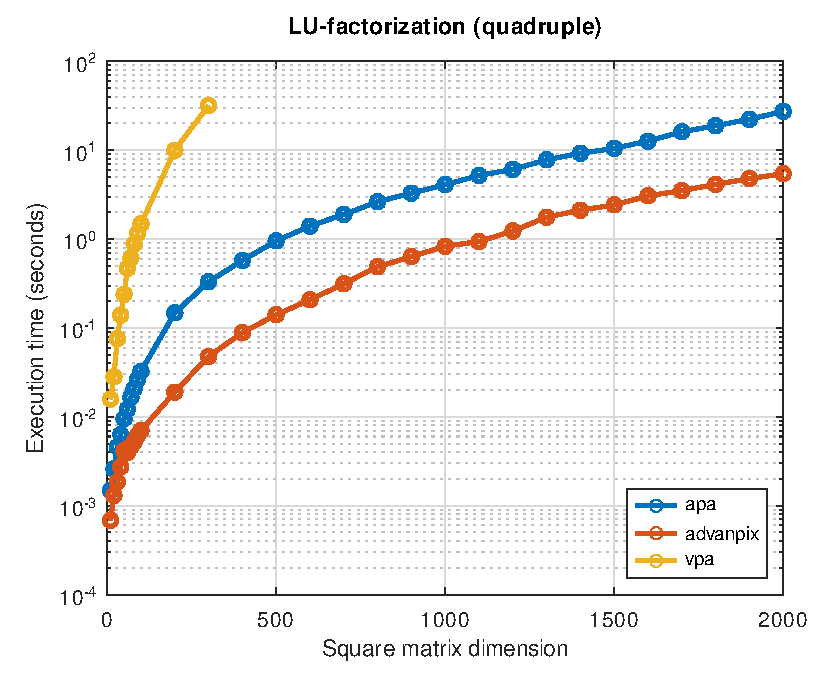
\includegraphics[width=1.0\linewidth]{res/data/2021-11-24_run-01-lu-quadruple-semilogy}
\end{figure}
\end{column}
\begin{column}{0.3\textwidth}
\begin{figure}
\centering
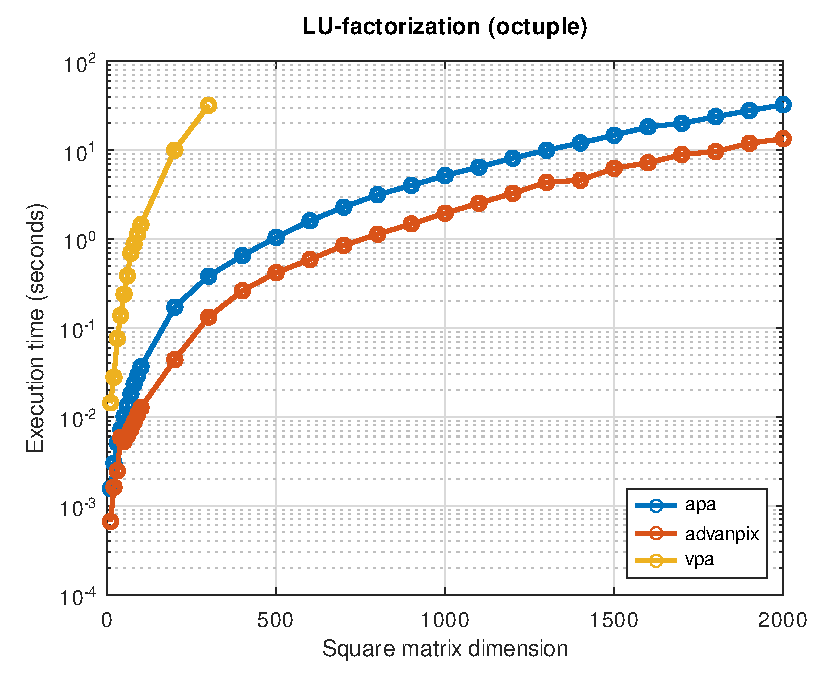
\includegraphics[width=1.0\linewidth]{res/data/2021-11-24_run-01-lu-octuple-semilogy}
\end{figure}
\end{column}
\end{columns}

\end{frame}


\begin{frame}{Benchmark (4/4)}

\begin{columns}
\begin{column}{0.3\textwidth}
\begin{figure}
\centering
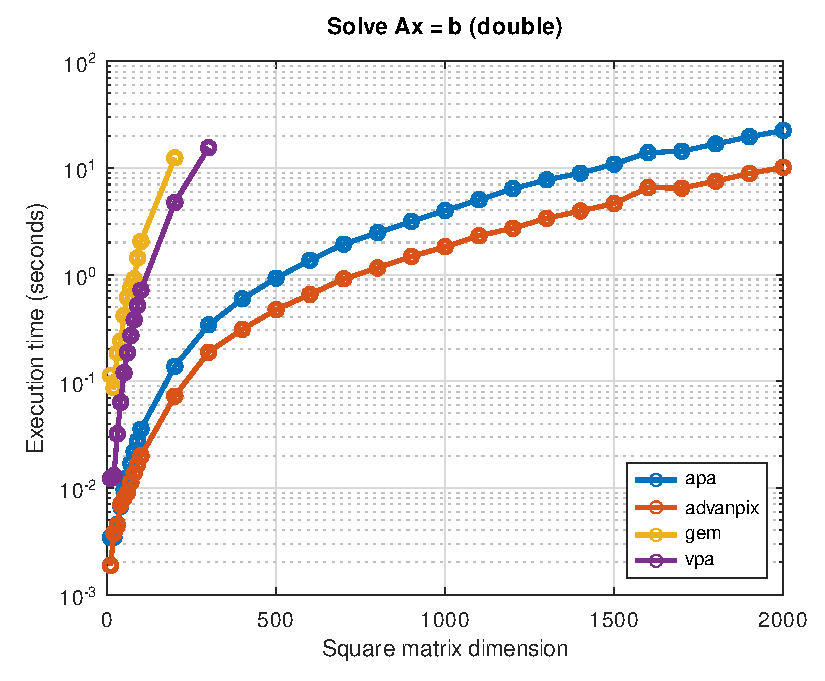
\includegraphics[width=1.0\linewidth]{res/data/2021-11-24_run-01-lin-double-semilogy}
\end{figure}
\end{column}
\begin{column}{0.3\textwidth}
\begin{figure}
\centering
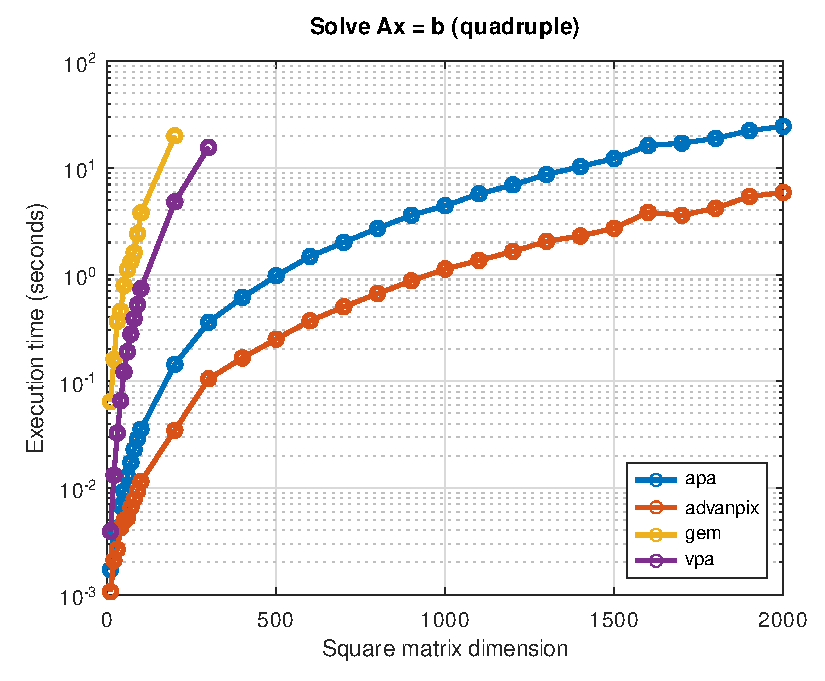
\includegraphics[width=1.0\linewidth]{res/data/2021-11-24_run-01-lin-quadruple-semilogy}
\end{figure}
\end{column}
\begin{column}{0.3\textwidth}
\begin{figure}
\centering
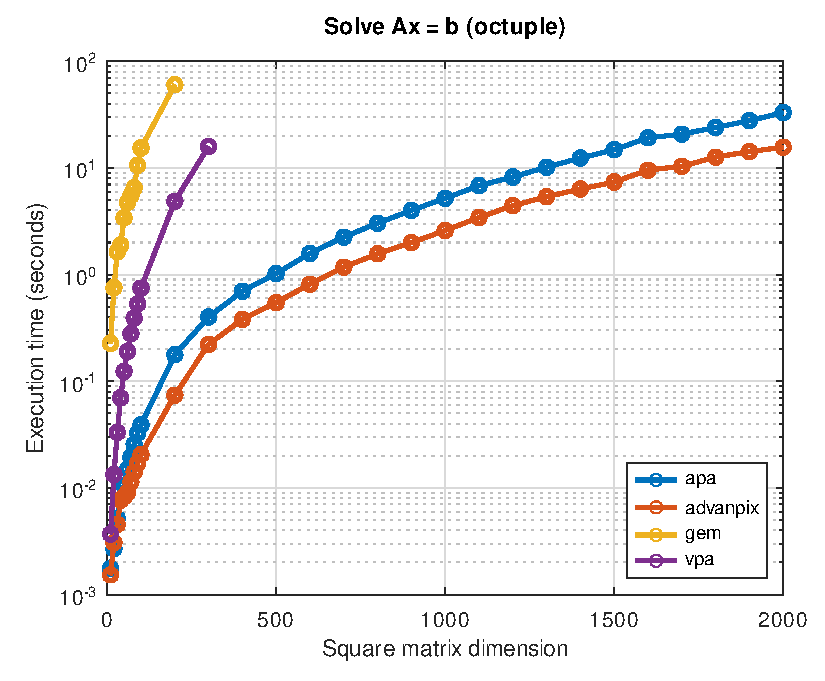
\includegraphics[width=1.0\linewidth]{res/data/2021-11-24_run-01-lin-octuple-semilogy}
\end{figure}
\end{column}
\end{columns}

\end{frame}